\documentclass{beamer}

% Title page details:
\title{Exercise 1}
\subtitle{Kepler Orbits}
\date{\today}

\begin{document}

% Title page frame
\begin{frame}
    \titlepage
\end{frame}

\begin{frame}{Nsteps}

	Comparison between different nsteps $10^2$ to $10^5$ ($dt = \frac{T}{nsteps}$)

\begin{figure}
\centering
    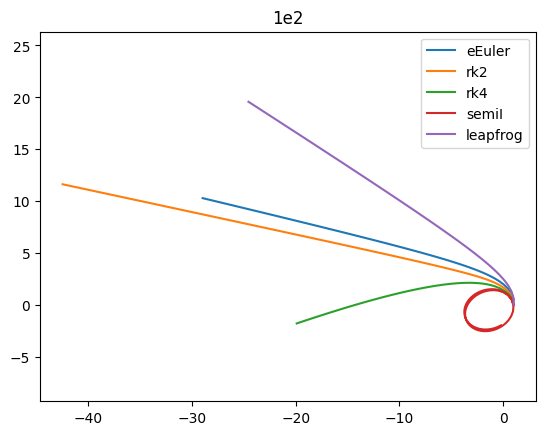
\includegraphics[width=0.4\textwidth]{../plots/1e2_plot.png}
    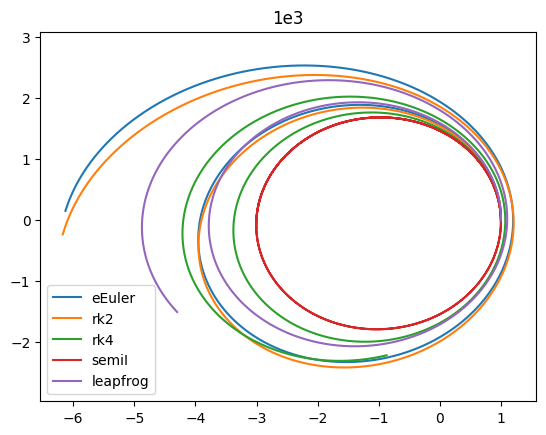
\includegraphics[width=0.4\textwidth]{../plots/1e3_plot.png}
    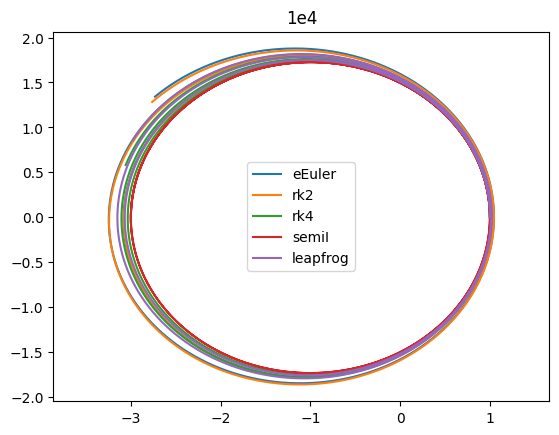
\includegraphics[width=0.4\textwidth]{../plots/1e4_plot.png}
    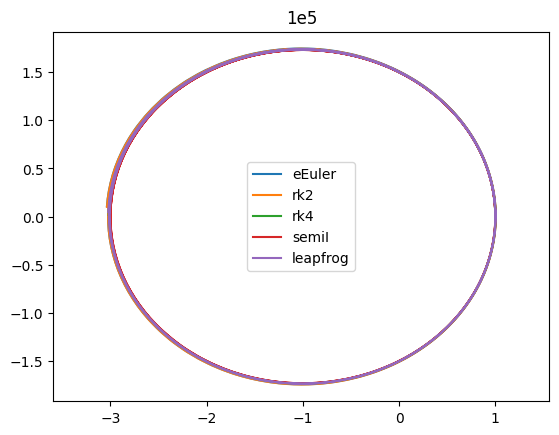
\includegraphics[width=0.4\textwidth]{../plots/1e5_plot.png}
    \label{fig:question}
\end{figure}
\end{frame}

\begin{frame}{Eccentricity}

	Comparison between different eccentricity values $0.1$ to $0.9$

\begin{figure}
\centering
    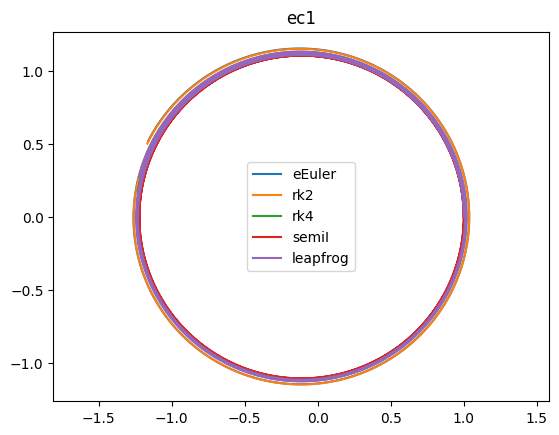
\includegraphics[width=0.4\textwidth]{../plots/ec1_plot.png}
    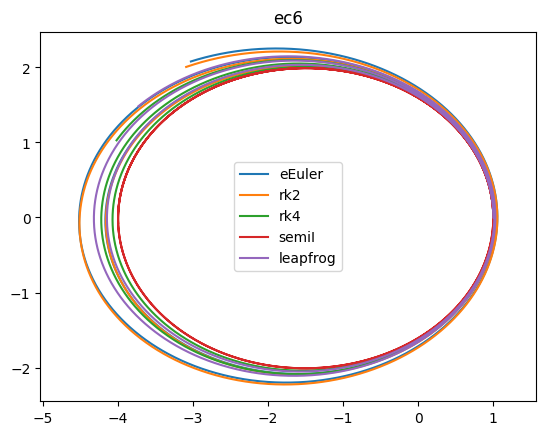
\includegraphics[width=0.4\textwidth]{../plots/ec6_plot.png}
    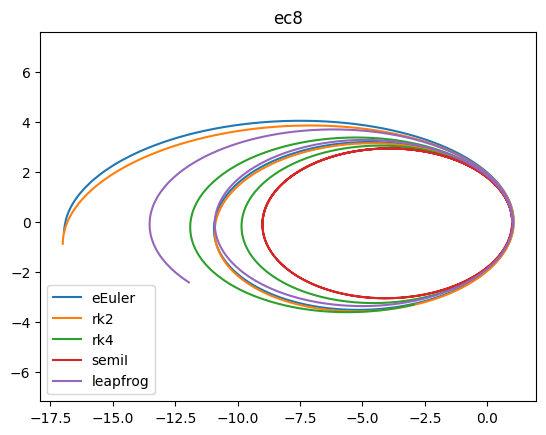
\includegraphics[width=0.4\textwidth]{../plots/ec8_plot.png}
    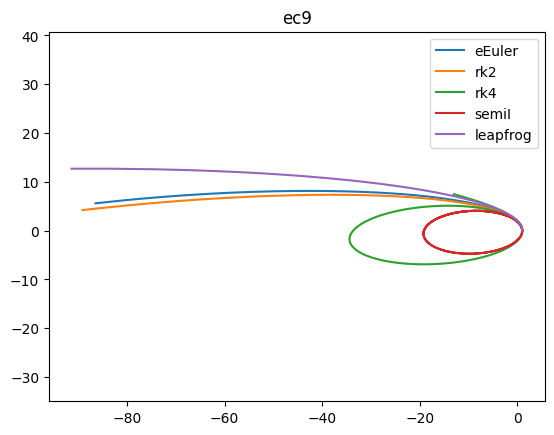
\includegraphics[width=0.4\textwidth]{../plots/ec9_plot.png}
    \label{fig:question}
\end{figure}
\end{frame}
\begin{frame}{Summary}

For low values of nsteps $10^2$ and $10^3$ the integration methods produce considerably different results. \bigskip

With increasing nsteps these differences tend to disappear. \bigskip

For the eccentricity, it is true the opposite, with lower eccentricity we have similar results.\bigskip

The Semi Implicit Euler scheme seems to perform well with all the range of values tried, both for varying eccentricity as for varying nsteps.

\end{frame}
\begin{frame}{Validation}

	Energy and Momentum delta along $10^4$ steps ($1 T$)
\begin{figure}
\centering
    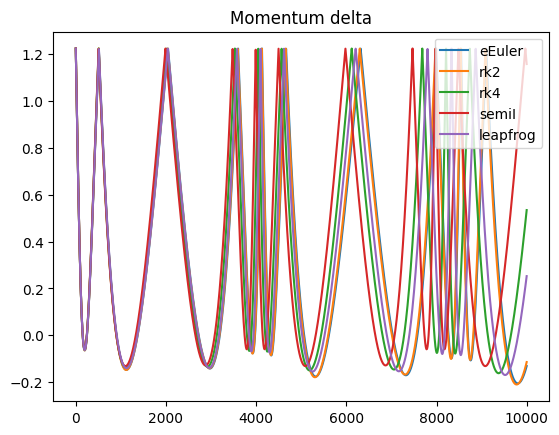
\includegraphics[width=0.4\textwidth]{../plots/plot_M.png}
    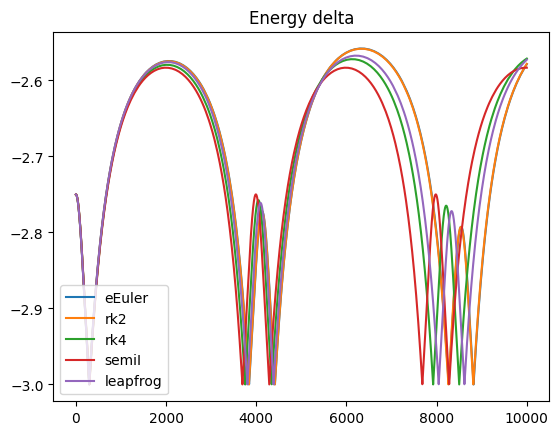
\includegraphics[width=0.4\textwidth]{../plots/plot_E.png}
    \label{fig:question}
\end{figure}
The plots are very similar between different numerical methods.
This might suggest there is a problem, not all of these methods are supposed to behave in the same way.
\end{frame}

\begin{frame}{Benchmark}
Performance in $GFlops/s$ ($P = \frac{Op}{\Delta t} \cdot 10^{-9}$)
\begin{figure}
	\centering
	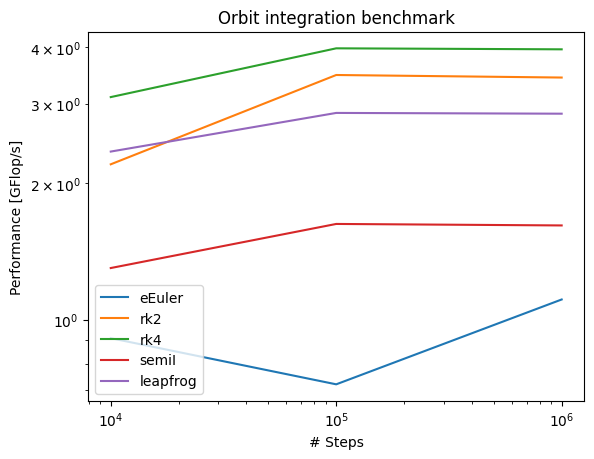
\includegraphics[width = 0.7\textwidth]{../plots/benchmark_plot.png}
\end{figure}
\end{frame}
\end{document}
